\documentclass[12pt]{article}
\usepackage{sbc-template}
\usepackage[T1]{fontenc}
\usepackage[utf8]{inputenc}
\usepackage{babel}
\babelprovide[import,main]{portuguese}
\usepackage{graphicx,booktabs,microtype}
\usepackage[hidelinks]{hyperref}
\hypersetup{pdftitle={Idade ossea pediatrica com descritores manuais},pdfauthor={Carlos Daniel Reis da Silva; Raul Ferreira Holanda; Rílari Maia Castelo},pdfsubject={CV, teste e analise OOF - versao para revisao},pdflang={pt-BR}}
\urlstyle{same}
\emergencystretch=2em
\renewcommand{\refname}{Referências}
\renewcommand{\figurename}{Figura}
\renewcommand{\tablename}{Tabela}
\title{Idade óssea pediátrica com descritores manuais:\\comparação de regressores clássicos}
\author{Carlos Daniel Reis da Silva, Raul Ferreira Holanda, Rílari Maia Castelo}
\address{Sistemas de Informação\\
UniCatólica -- Centro Universitário Católica de Quixadá\\
Quixadá -- CE -- Brasil
\email{reisdaniel739@gmail.com, raulfholanda@gmail.com}\\\texttt{2023010247@unicatolicaquixada.edu.br}}
\date{}
\begin{document}
\maketitle
\begin{resumo}
Comparamos descritores manuais para estimar idade óssea na base RSNA. Uma amostra de 4.000 imagens recebeu IDs congelados de treino, validação e teste. Três dobras nos 2.800 casos de treino compararam textura, HOG e intensidade, com sexo como covariável. HOG com Gradient Boosting obteve MAE de $22{,}21\pm0{,}85$ meses na CV e 22,14 nos 600 casos de teste, contra 33,69 da média do treino. Reduzir a resolução da textura de 224 para 128 pixels aumentou o MAE interno em 0,73 mês. Os erros OOF foram maiores nas idades extremas. A independência por paciente não foi verificada.
\end{resumo}
\begin{abstract}
We compare handcrafted descriptors for RSNA bone age estimation. A 4,000-image sample received frozen training, validation and test IDs. Three folds within 2,800 training cases compared texture, HOG and intensity, with sex as a covariate. HOG with Gradient Boosting achieved a mean MAE of $22.21\pm0.85$ months in CV and 22.14 on 600 test cases, versus 33.69 for the training-mean baseline. Reducing texture resolution from 224 to 128 pixels increased internal MAE by 0.73 months. OOF errors were larger at the age extremes. Patient independence was not verified.
\end{abstract}
\section{Introdução}
A estimativa de maturidade esquelética em radiografias pediátricas de mão é a tarefa do desafio RSNA \cite{halabi}. Formulamos a idade óssea, em meses, como regressão a partir da imagem e do sexo. Um baseline com características explícitas permite comparar representações antes de desenvolver modelos mais complexos. As contribuições são:
\begin{itemize}
\item amostra auditada e IDs congelados com pré-processamento comum;
\item comparação de três famílias e três regressores, com baseline trivial;
\item ablação de resolução e análise de previsões fora da dobra (OOF).
\end{itemize}
\section{Trabalhos relacionados}
Halabi et al. \cite{halabi} situam o desafio RSNA, e Larson et al. \cite{larson} investigam redes profundas para maturidade esquelética. Nosso estudo privilegia descritores explícitos e não compara diretamente números de protocolos distintos. GLCM \cite{haralick} e LBP \cite{ojala} representam textura; HOG \cite{dalal}, desenvolvido para detecção humana, representa gradientes. Sua aplicação à idade óssea é uma hipótese experimental. SVR \cite{smola}, Random Forest \cite{breiman} e Gradient Boosting \cite{friedman} oferecem modelos distintos para a mesma representação. A seleção pela própria CV pode favorecer estimativas otimistas \cite{varma}; por isso, distinguimos desenvolvimento de avaliação externa.
\newpage
\section{Metodologia}
\textbf{Dados e protocolo.} A versão 2 de \texttt{kmader/rsna-bone-age} contém 12.611 imagens, idades de 1 a 228 meses e 5.778 rótulos femininos e 6.833 masculinos. Para limitar o custo, amostramos 4.000 imagens, semente 42, por sexo e faixas $[0,72)$, $[72,132)$, $[132,192)$ e $[192,240)$ meses. Congelamos 2.800 IDs de treino, 600 de validação e 600 de teste. São divisões do treino público com IDs disjuntos. \textbf{Não há chave verificável de paciente}: o protocolo por imagem é provisório e não comprova agrupamento por paciente.

\textbf{Pixels comuns.} Usamos cinza (Pillow L), $224\times224$ com Lanczos e divisão por 255 em \texttt{float32}, sem recorte, remoção de fundo ou realce. A ablação examina essa resolução operacional.

\textbf{Representações.} Textura combina LBP uniforme \cite{ojala}, oito pontos e raio um (histograma de dez valores), com GLCM \cite{haralick} de 16 níveis, distâncias 1 e 2 e ângulos $0^\circ$, $45^\circ$, $90^\circ$, $135^\circ$, simétrica e normalizada. Média e desvio populacional de contraste, dissimilaridade, homogeneidade, energia e correlação nos oito pares produzem dez atributos. HOG \cite{dalal} usa nove orientações, células $16\times16$, blocos $2\times2$ e normalização L2-Hys (6.084 atributos). Intensidade usa histograma de 32 intervalos em $[0,1]$, densidade, média, desvio e percentis 25, 50 e 75 (37 atributos). Sexo é acrescentado a todas as famílias; a média adicional do extrator de textura é excluída.

\textbf{Ajuste e avaliação.} Com scikit-learn \cite{pedregosa}, comparamos configurações fixas: SVR RBF ($C=10$, $\epsilon=1$, $\gamma=\mathrm{scale}$); RF, 300 árvores, profundidade ilimitada e todas as características; GB, 300 estimadores, profundidade três e taxa 0,05. Árvores usam semente 42. Três dobras estratificadas por idade e sexo, embaralhadas com semente 42, têm 934, 933 e 933 casos. StandardScaler é ajustado apenas no treino de cada dobra; o baseline prediz sua média de idades. A seleção pela mesma CV não é avaliação independente \cite{varma}. MAE e RMSE medem erro em meses; $R^2$ mede variação explicada. Reportamos média e desvio amostral entre dobras. O teste registrado usa os mesmos parâmetros, fixados antes do acesso, treino de 2.800 casos e scaler ajustado apenas nele; avalia 600 casos, sem incorporar a validação ao treino final.

A ablação compara textura em 224 e 128 pixels, mantendo GB, sexo e dobras. Código, IDs, parâmetros e resultados: \url{https://github.com/RaulFH0/tp1-e2-bone-age}. O teste foi publicado por Raul em \texttt{e3b12d7}; as figuras usam apenas previsões OOF.
\begin{figure}[!h]
\centering
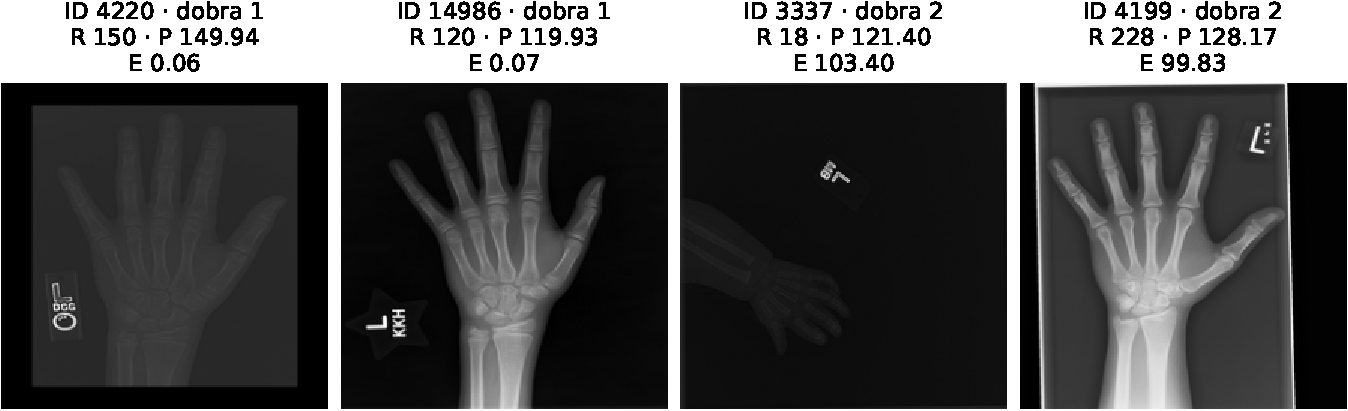
\includegraphics[width=\linewidth]{figuras/casos_oof.pdf}
\caption{Casos OOF em pixels comuns: dois menores erros e maiores erros nas faixas 0--5 e 16--19 anos. R: referência; P: previsão; E: erro absoluto, em meses.}
\label{fig:casos}
\end{figure}
\newpage
\section{Resultados e discussão}
A Tabela~\ref{tab:cv} distingue a CV de desenvolvimento do teste registrado. HOG+GB, candidato com menor MAE na CV, obteve 22,14 meses no teste, redução de 34,28\% contra o baseline de 33,69. O registro informa avaliação única, sem ajuste posterior; não realizamos teste de significância. Na ablação interna, 128 pixels aumentou o MAE em 0,73 mês; diferenças por dobra: 0,01, 1,28 e 0,91.
\begin{table}[!h]
\centering
\caption{CV: MAE médio $\pm$ desvio em três dobras; teste: métricas nos 600 casos. MAE/RMSE em meses; RF: Random Forest; GB: Gradient Boosting.}
\label{tab:cv}
\setlength{\tabcolsep}{3pt}
\begin{tabular}{llrrrr}
\toprule
Família & Modelo & MAE CV & MAE teste & RMSE teste & $R^2$ teste\\
\midrule
Baseline & Média & $33{,}83\pm0{,}99$ & $33{,}69$ & $40{,}85$ & $-0{,}0003$\\
Textura 224 & SVR & $25{,}71\pm0{,}41$ & $25{,}17$ & $32{,}34$ & $0{,}373$\\
 & RF & $24{,}84\pm0{,}93$ & $24{,}50$ & $31{,}39$ & $0{,}409$\\
 & GB & $24{,}81\pm0{,}98$ & $24{,}16$ & $31{,}34$ & $0{,}411$\\
HOG & SVR & $28{,}15\pm0{,}89$ & $27{,}21$ & $33{,}96$ & $0{,}309$\\
 & RF & $26{,}73\pm0{,}99$ & $26{,}36$ & $33{,}01$ & $0{,}347$\\
 & GB & $\mathbf{22{,}21\pm0{,}85}$ & $\mathbf{22{,}14}$ & $28{,}29$ & $0{,}520$\\
Intensidade & SVR & $28{,}35\pm0{,}74$ & $26{,}96$ & $35{,}15$ & $0{,}259$\\
 & RF & $25{,}76\pm1{,}18$ & $24{,}73$ & $31{,}92$ & $0{,}389$\\
 & GB & $25{,}95\pm1{,}04$ & $24{,}91$ & $32{,}02$ & $0{,}385$\\
Textura 128 & GB & $25{,}54\pm1{,}51$ & -- & -- & --\\
\bottomrule
\end{tabular}
\end{table}

Nas 2.800 previsões OOF de HOG+GB, Bland--Altman \cite{bland} apresenta viés de $+0{,}22$ mês e limites descritivos de $-55{,}38$ e $+55{,}81$ (predito menos referência; média $\pm1{,}96$ DP). O viés pequeno oculta superestimação nas idades menores e subestimação nas maiores (Figura~\ref{fig:erro}); não demonstra concordância clínica.
\begin{figure}[!h]
\centering
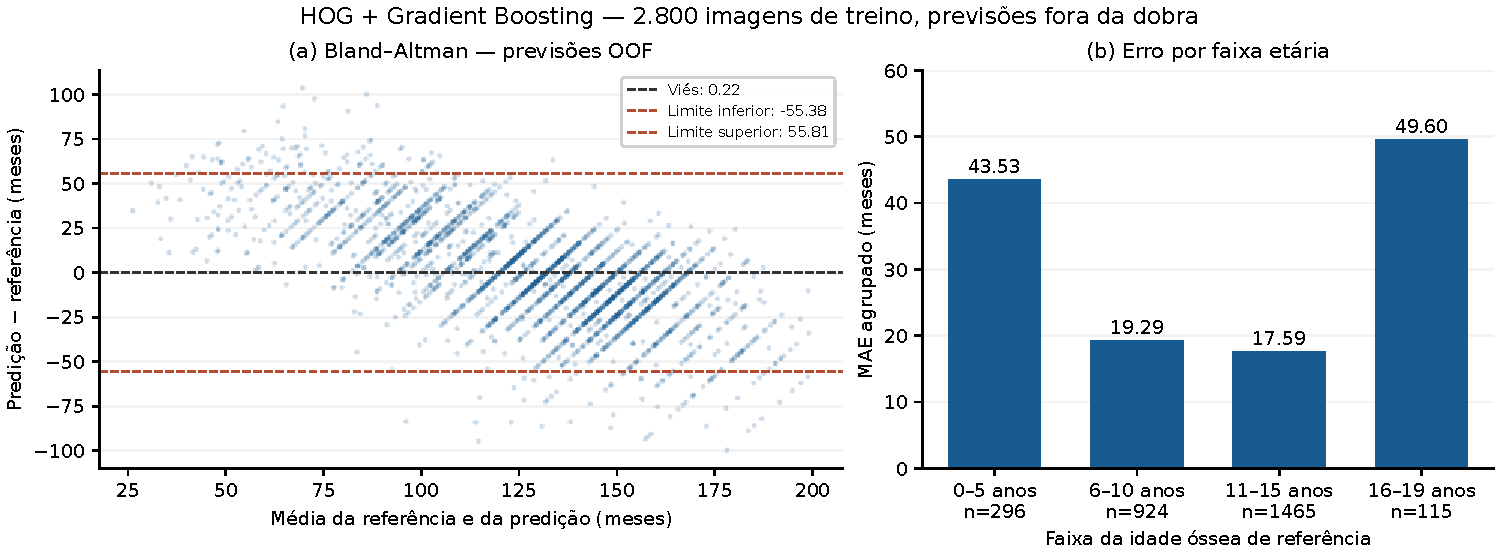
\includegraphics[width=\linewidth]{figuras/erro_oof.pdf}
\caption{HOG+GB: Bland--Altman e MAE por faixa, agrupados sobre previsões OOF; barras identificam o número de casos.}
\label{fig:erro}
\end{figure}

\newpage
\section{Conclusão}
HOG+GB, selecionado pela CV, alcançou MAE de 22,14 meses no teste registrado; textura favoreceu 224 pixels na ablação interna. Os extremos etários tiveram maior erro e menor representação. Na Figura~\ref{fig:casos}, 3337 tem pouca luminosidade e enquadramento deslocado, mas 4220 também é escuro e apresenta erro pequeno: aparência não estabelece causalidade. A seleção ilustrativa não é aleatória. A ausência de chave de paciente, a amostragem e a escolha pela mesma CV limitam a generalização. São próximos passos esclarecer o agrupamento e avaliar melhorias em outro protocolo, preservando o teste já utilizado de novos ajustes. Estes resultados não validam uso clínico.

\begin{thebibliography}{11}
\bibitem{halabi} Halabi, S. S. et al. (2019). \href{https://doi.org/10.1148/radiol.2018180736}{The RSNA Pediatric Bone Age Machine Learning Challenge.} \textit{Radiology}, 290(2):498--503.
\bibitem{larson} Larson, D. B. et al. (2018). \href{https://doi.org/10.1148/radiol.2017170236}{Performance of a Deep-Learning Neural Network Model in Assessing Skeletal Maturity on Pediatric Hand Radiographs.} \textit{Radiology}, 287(1):313--322.
\bibitem{haralick} Haralick, R. M., Shanmugam, K. e Dinstein, I. (1973). \href{https://doi.org/10.1109/TSMC.1973.4309314}{Textural Features for Image Classification.} \textit{IEEE Trans. Syst., Man, Cybern.}, SMC-3(6):610--621.
\bibitem{ojala} Ojala, T., Pietikäinen, M. e Mäenpää, T. (2002). \href{https://doi.org/10.1109/TPAMI.2002.1017623}{Multiresolution Gray-Scale and Rotation Invariant Texture Classification with Local Binary Patterns.} \textit{IEEE Trans. Pattern Anal. Mach. Intell.}, 24(7):971--987.
\bibitem{dalal} Dalal, N. e Triggs, B. (2005). \href{https://doi.org/10.1109/CVPR.2005.177}{Histograms of Oriented Gradients for Human Detection.} \textit{CVPR}, 1:886--893.
\bibitem{smola} Smola, A. J. e Schölkopf, B. (2004). \href{https://doi.org/10.1023/B:STCO.0000035301.49549.88}{A tutorial on support vector regression.} \textit{Statistics and Computing}, 14:199--222.
\bibitem{breiman} Breiman, L. (2001). \href{https://doi.org/10.1023/A:1010933404324}{Random Forests.} \textit{Machine Learning}, 45:5--32.
\bibitem{friedman} Friedman, J. H. (2001). \href{https://doi.org/10.1214/aos/1013203451}{Greedy function approximation: A gradient boosting machine.} \textit{The Annals of Statistics}, 29(5):1189--1232.
\bibitem{varma} Varma, S. e Simon, R. (2006). \href{https://doi.org/10.1186/1471-2105-7-91}{Bias in error estimation when using cross-validation for model selection.} \textit{BMC Bioinformatics}, 7:91.
\bibitem{bland} Bland, J. M. e Altman, D. G. (1986). \href{https://doi.org/10.1016/S0140-6736(86)90837-8}{Statistical methods for assessing agreement between two methods of clinical measurement.} \textit{The Lancet}, 327(8476):307--310.
\bibitem{pedregosa} Pedregosa, F. et al. (2011). \href{https://www.jmlr.org/papers/v12/pedregosa11a.html}{Scikit-learn: Machine Learning in Python.} \textit{Journal of Machine Learning Research}, 12:2825--2830.
\end{thebibliography}
\noindent\textbf{Apoio de IA.} IA generativa auxiliou revisão de código, elaboração de testes, organização do texto e tradução do abstract. Resultados e referências exigem conferência pelos autores; a responsabilidade pela versão submetida permanece com a equipe.
\end{document}
